\subsection{Controlador PID}

Com base nas análises conduzidas na Atividade 4, foi estabelecido um valor limite para o ganho crítico, \( K_c \), de 14.93. Este parâmetro é crucial para o ajuste dos parâmetros do controlador PID utilizando o método de Ziegler-Nichols. Semelhante ao procedimento adotado na Atividade 5, simulou-se o comportamento do sistema com um sinal de entrada em forma de degrau, cuja amplitude é definida como \( A = \frac{m}{4} \). Considerando que \( m = 10 \), a amplitude do degrau é \( A = 2.5 \). Este cenário permitiu a observação direta das respostas do sistema sob o efeito do ganho crítico.

\begin{figure}[H]
    \centering
    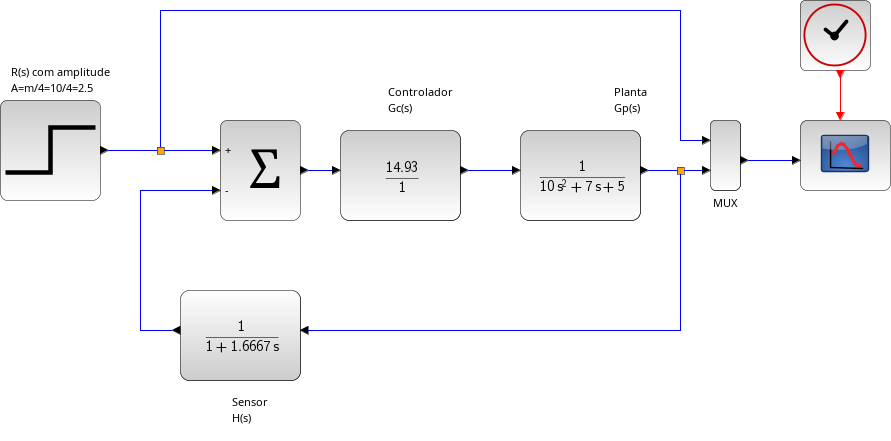
\includegraphics[width=0.7\textwidth]{atividades/6-atividade/assets/a/diagrama-ganho-critico-sistema-instavel.png}
    \caption{Diagrama mostrando o sistema no ponto crítico com \( K_c = 14.93 \)}
    \label{fig:diagrama-ponto-critico}
\end{figure}

A simulação realizada no ganho crítico, \( K_c = 14.93 \), demonstra que o sistema atinge uma condição de oscilação não amortecida, o que é indicativo de uma fronteira entre a estabilidade e a instabilidade. Essa observação é fundamental, pois o ponto de oscilação não amortecida é usado pelo método de Ziegler-Nichols para calibrar os controladores PID, visando uma resposta rápida e minimamente oscilatória em regime permanente.

\begin{figure}[H]
    \centering
    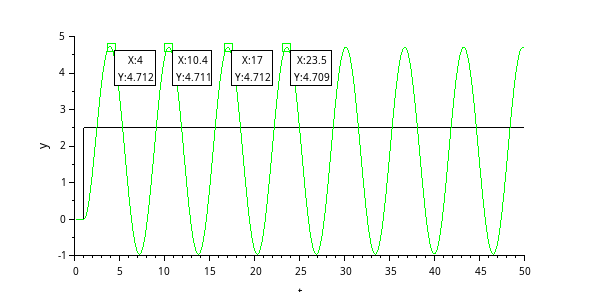
\includegraphics[width=0.7\textwidth]{atividades/6-atividade/assets/a/ganho-critico-sistema-instavel.png}
    \caption{Resposta do sistema com o controlador PID ajustado para \( K_c = 14.93 \)}
    \label{fig:ganho-critico-sistema-instavel}
\end{figure}


Como observado no gráfico de resposta temporal, o sistema exibe oscilações contínuas com uma amplitude aproximadamente constante, confirmando a caracterização do ganho crítico. Esta condição é explorada para determinar o período crítico \( P_c \), calculado pela medição do intervalo entre picos consecutivos. O valor de \( P_c \) é crucial para definir os parâmetros do controlador PID, pois influencia diretamente a dinâmica de correção implementada pelo controlador.

Os dados obtidos deste experimento são essenciais para a calibração dos parâmetros do controlador PID. Ajustar o controlador para operar próximo do ponto crítico, mas com garantias de estabilidade, permite aproveitar a máxima capacidade de resposta do sistema sem comprometer sua segurança operacional. Esta abordagem visa melhorar tanto a eficiência quanto a estabilidade do sistema, tornando o controle mais robusto frente a variações nas condições operacionais.

\subsubsection{Determinação do Período Crítico}
O período crítico \( P_c \) foi determinado a partir da análise do gráfico de resposta em regime oscilatório no ganho crítico. Identificamos os picos consecutivos e medimos o tempo entre eles para calcular o \( P_c \). A partir dos pontos identificados no gráfico, com os tempos \( t_1 = 9.98 \, \text{s} \) e \( t_2 = 16.894 \, \text{s} \), o período crítico foi calculado como:
\[
    P_c = t_2 - t_1 = 16.894 - 9.98 = 6.914 \, \text{s}
\]
Este valor é importante para o ajuste subsequente dos parâmetros do controlador PID utilizando o método de Ziegler-Nichols.


\subsubsection{Determinação dos Parâmetros do Controlador PID}
Após identificarmos o ganho crítico \( K_c = 14.93 \) através de análises detalhadas, empregamos o método de Ziegler-Nichols para ajustar os parâmetros do controlador PID. Este método é eficaz para sintonizar controladores em sistemas onde a resposta precisa ser otimizada em termos de estabilidade e rapidez.

\subsubsection{Cálculo dos Parâmetros do Controlador PID}
O método de Ziegler-Nichols, conhecido por sua eficiência na configuração inicial de controladores PID, utiliza o ganho crítico \( K_c \) e o período crítico \( P_c \) para estabelecer os parâmetros de controle, ajustando assim a resposta do sistema.

\begin{itemize}
    \item \textbf{Ganho Proporcional} \( K_p \):
          \[
              K_p = 0.6 \times K_c = 0.6 \times 14.93 = 8.958
          \]
    \item \textbf{Ganho Integral} \( K_i \):
          \[
              K_i = \frac{2}{P_c} = \frac{2}{6.914} \approx 0.289
          \]
    \item \textbf{Ganho Derivativo} \( K_d \):
          \[
              K_d = 0.125 \times P_c = 0.125 \times 6.914 = 0.864
          \]
\end{itemize}

\subsubsection{Implementação e Validação dos Parâmetros}
Os parâmetros \( K_p = 8.958 \), \( K_i = 0.289 \), e \( K_d = 0.864 \) são implementados no controlador PID no ambiente de simulação Scilab. Esses valores são projetados para ajustar o sistema a fim de responder de forma ideal em diversas condições operacionais, melhorando tanto a estabilidade quanto a precisão do sistema.

A eficácia desses parâmetros será validada por meio de simulações adicionais, que irão confirmar se eles conseguem manter o desempenho desejado do sistema, assegurando que o controle PID seja eficiente e eficaz.

\begin{figure}[H]
    \centering
    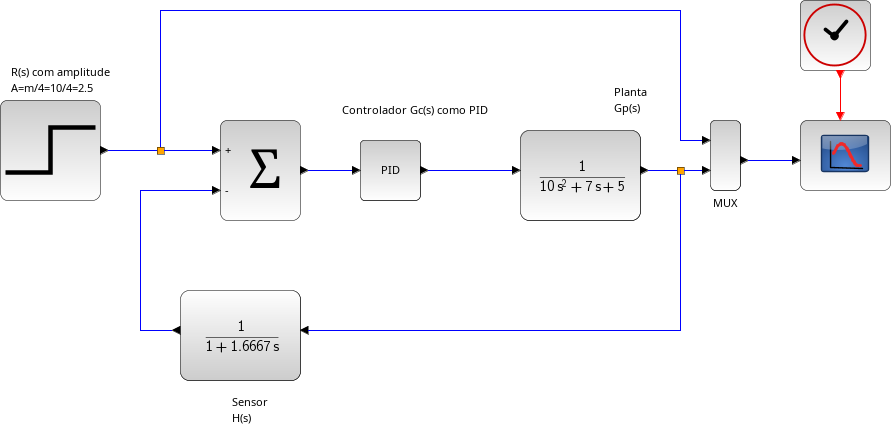
\includegraphics[width=0.8\textwidth]{atividades/6-atividade/assets/a/diagrama-pid.png}
    \caption{Resposta do sistema com os parâmetros do PID ajustados.}
    \label{fig:diagrama-pid}
\end{figure}

\begin{figure}[H]
    \centering
    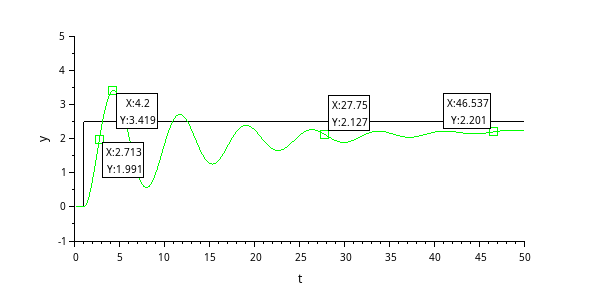
\includegraphics[width=0.8\textwidth]{atividades/6-atividade/assets/a/pid.png}
    \caption{Resposta do sistema com os parâmetros do PID ajustados.}
    \label{fig:resposta-pid}
\end{figure}

Após a validação inicial, pode ser necessário um refinamento manual dos parâmetros para otimizar ainda mais a resposta do sistema. Este processo de ajuste fino baseia-se na análise detalhada das respostas obtidas e na experiência prática, permitindo uma sintonia mais precisa que se adapta adequadamente às especificidades do sistema e às variações nas condições operacionais. Este ajuste é crucial para alcançar o melhor equilíbrio entre estabilidade e rapidez na resposta do controlador PID.

Subsequentemente, novas simulações serão realizadas para validar a eficácia dos parâmetros ajustados. Esta etapa é fundamental para verificar se os ajustes refinados mantêm a saída do sistema próxima ao valor desejado sob uma gama mais ampla de condições operacionais, garantindo a eficácia e a eficiência do controle.